\documentclass{article}

% if you need to pass options to natbib, use, e.g.:
% \PassOptionsToPackage{numbers, compress}{natbib}
% before loading nips_2018

% ready for submission
\usepackage{nips_2018}

% to compile a preprint version, e.g., for submission to arXiv, add
% add the [preprint] option:
%\usepackage[preprint]{nips_2018}

% to compile a camera-ready version, add the [final] option, e.g.:
%\usepackage[final]{nips_2018}

% to avoid loading the natbib package, add option nonatbib:
%\usepackage[nonatbib]{nips_2018}

\usepackage[utf8]{inputenc} % allow utf-8 input
\usepackage[T1]{fontenc}    % use 8-bit T1 fonts
\usepackage{hyperref}       % hyperlinks
\usepackage{url}            % simple URL typesetting
\usepackage{booktabs}       % professional-quality tables
\usepackage{amsfonts}       % blackboard math symbols
\usepackage{nicefrac}       % compact symbols for 1/2, etc.
\usepackage{microtype}      % microtypography
\usepackage{xcolor}
\usepackage{graphicx}

\title{ParamNet: Towards A Network of \emph{Parameterization Prediction} for Shape Generation from a Single Image}

% The \author macro works with any number of authors. There are two
% commands used to separate the names and addresses of multiple
% authors: \And and \AND.
%
% Using \And between authors leaves it to LaTeX to determine where to
% break the lines. Using \AND forces a line break at that point. So,
% if LaTeX puts 3 of 4 authors names on the first line, and the last
% on the second line, try using \AND instead of \And before the third
% author name.

\author{
  David S.~Hippocampus\thanks{Use footnote for providing further
    information about author (webpage, alternative
    address)---\emph{not} for acknowledging funding agencies.} \\
  Department of Computer Science\\
  Cranberry-Lemon University\\
  Pittsburgh, PA 15213 \\
  \texttt{hippo@cs.cranberry-lemon.edu} \\
  %% examples of more authors
  %% \And
  %% Coauthor \\
  %% Affiliation \\
  %% Address \\
  %% \texttt{email} \\
  %% \AND
  %% Coauthor \\
  %% Affiliation \\
  %% Address \\
  %% \texttt{email} \\
  %% \And
  %% Coauthor \\
  %% Affiliation \\
  %% Address \\
  %% \texttt{email} \\
  %% \And
  %% Coauthor \\
  %% Affiliation \\
  %% Address \\
  %% \texttt{email} \\
}

\begin{document}
% \nipsfinalcopy is no longer used

\maketitle

\begin{abstract}
	Self-intersection in surfaces is a typical defect that makes a 3D model unsuitable for many applications. 
	Existing neural networks for 3D mesh reconstruction has the challenges of integrating self-intersection prevention in their unidirectional frameworks.
	In this paper, we propose to use cycle regularization as a self-intersection prevention technique for mesh reconstruction networks.
	It is flexible to integrate into networks for generating meshes. Our experiments on two latest mesh reconstruction networks demonstrates that the proposed cycle regularization can effectively reduce the self-intersection in generated mesh while remains similar discrepancy with target surface 
\end{abstract}
\section{Introduction}
\begin{figure}[htbp]
	\centering
	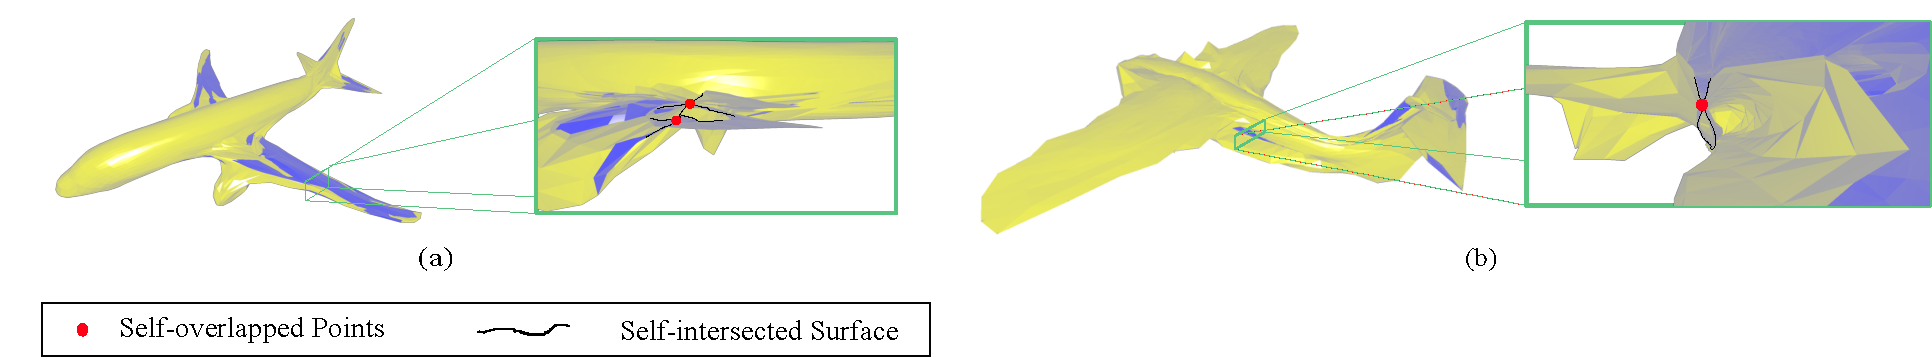
\includegraphics[width=\linewidth]{img/issue/issue}
	\caption{Self-intersections in 3D surface mesh reconstruction networks. (a) A surface mesh of a plane generated by AtlasNet \cite{atlasnet} (sphere as its parameter domain). (b) A surface mesh of a plane generated by Pixel2Mesh \cite{pixel2mesh}. Outside faces are rendered as golden and inside faces are rendered as bluish. \mdf{Some} inside triangles are exposed due to self-intersections. We highlight some self-intersected faces and their corresponding overlapped points in the close-up view.}
	\label{fig:issue}
\end{figure}
%introduction to 3D shape reconstruction from single view
Inferring 3D shape from a single view image is a traditional problem for computer vision. In computer graphics, 3D modeling \mdf{from} a given image has also been extensively studied. In recent years, deep neural networks (\cite{3DR2N2,PSGN,3Drender,imgrecon15,3dshapenet,endface,octreegen,surfnet,shapeprior}) have achieved great success in this field. Unlike classic shape from X (e.g. \cite{shapefromshading,shapefromtext1,shapefromtext2}) approaches, these neural networks are able to recover not only the visible frontal shape but also the invisible part for an object from a single-view color image by learning and representing complicated prior knowledge from a large dataset. 

Existing networks all rely on variants of 2D convolution neural networks to extract information and encode 2D images, but use quite different techniques to represent and decode 3D shapes. Started from 3D ShapeNets \cite{3dshapenet} and greatly improved by introducing octree structure (\cite{octreegen}), volumetric representation and 3D convolutional networks are most commonly used in this problem. A point set generation network (\cite{PSGN}) use unordered point set representation and directly regresses a point set using both convolutional and fully connected branches. \cite{endface} employ a bilinear model to represent 3D faces and regress the interpolation coefficients to generate a face shape from one image. \cite{surfnet} explicitly use spherical parameterization as a post-processing stage to represent a 3D shape as a geometry image in the parameter domain. 

%introduction to 3d mesh reconstruction networks-- AtlasNet and Pixel2Mesh to be specific
In recent study, AtlasNet (\cite{atlasnet}) and Pixel2Mesh (\cite{pixel2mesh}) to be specific, a new idea has been applied on this problem. Neural networks are designed to learn the mapping from a predefined surface (square or sphere for AtlasNet, and ellipsoid for Pixel2Mesh) to a target surface instead of directly regressing the absolute positions of surface points as in \cite{PSGN}. These methods have shown great potential in generating meshes for generic objects. It is convenient to integrate mesh-related operations and energy functions in these networks. For example, Pixel2Mesh integrates graph-based unpooling and Laplacian regularization in the network.

Despite all of these progresses, there are still a number of issues such as how to increase shape details and  These issues prevent network-generated meshes from being praticable in many real-world applications. However, we believe deep learning is the most promising technique to integrate more intelligent methods in 3D modeling.

%introduction to the self-intersection issue
 In this paper, we address a specific issue that appears in both AtlasNet \cite{atlasnet} and Pixel2Mesh \cite{pixel2mesh}. As shown in Figure~\ref{fig:issue}, the AtlasNet and Pixel2Mesh frequently generate meshes with self-intersected surfaces. This issue appears partially because AtlasNet and Pixel2Mesh employ the Chamfer distance loss, which is used firstly to train the point set generation network (PSGN, \cite{PSGN}). The Chamfer distance loss was designed to measure the discrepancy between two unordered point sets and it does not take surface into consideration. AtlasNet uses Poission surface reconstruction as post-processing or double-sided lighting in rendering to cover up this issue. Pixel2Mesh adopts a coarse-to-fine framework and uses additional losses (i.e. edge length loss and Laplacian loss) in order to alleviate this issue. They all fail to address the essential reason behind this issue, while most efforts in these mesh generation networks have been put on increasing shape details for the generated meshes.

In this paper, we tackle the issue of self-intersection from the essential reason behind it, which is non-injectivity of the predicted mapping. Without injectivity, two points on the predefined surface could be possibly mapped to the same point by the neural network, which leads self-intersection or self-overlapping in the generated surface.
%challenge

\mdf{To enforce injectivity, one possible strategy is to start from a feasible solution and keep every deformation or optimization step inside feasible regions. In works of deformation (e.g. \cite{free-form-deform-solid,tvcgprevent}), such strategy is usually excuted as follows. A clean mesh that is free from self-intersection is chosen as intial mesh and local self-intersection is prevented by constraining the Jacobian of the mapping function in the following steps of the deformation. In works of parameterization optimization for surface with disk topology, the strategy is usually carried out by using Tutte's embedding \cite{tutte} or its variants to get a intial bijiective mapping and preventing triangle fold (preventing local self intersection) in following optimization steps. More specifically, triangle fold can be prevented by adding barrier energy from distortion metrics (e.g. \cite{provableplanarmapping,lifted_bijection}), bounding the triangle distortion (e.g.\cite{freeboundary,boundeddistortion}) or using a progressive strategy \cite{Liu_PP_2018}.}

It is non-trivial to adopt their strategies for training neural networks, since existing networks learn to predict the mapping for many different shapes simultaneously and only a batch of these shapes are sampled from the dataset in each training iteration. One challenge is to initialize the network parameters to ensure that initial outputs are free of self-intersection for all possible inputs. Another challenge is to alter batch-based optimizer to constrain the deformation of outputs within an injective region for all possible inputs. 

In order to learn injective mapping for meshes, we propose a cycle regularization technique. \mdf{Our technique is deduced from basic decision theorem of injectivity. It reduces not only local self-intersections but also global self-interferences of the surface.} It is easy to implement by reusing the existing differentiable layers within existing surface mesh reconstruction networks, such as AtlasNet \cite{atlasnet} and Pixel2Mesh \cite{pixel2mesh}.

%our solution
 Our strategy is to use an inverse 3D decoder to learn an inverse mapping from  the target surface back to the source surface along with the forward mapping in the original network. Therefore, a point from the source surface can be mapped to the target surface and then mapped back. We use the difference after such cycle mapping to form our regularization term and we call it cycle regularization. While the network learning a mapping to approximate the target surface, our regularization term \mdf{tries} to ensure that an inverse mapping exists (i.e. making the forward mapping injective, as we explain in Sec~\ref{subsec:cyclereg}).
Note that the inverse 3D decoder is only needed in the training phase. Therefore, it is a regularization technique which does not increase the complexity of the original neural network for mesh generation.

In summary, our contributions in this paper are three-fold.
\begin{itemize}
	\item We propose a novel cycle regularization technique to prevent self-intersection for surface mesh reconstruction networks. 
	\item We apply our cycle regularization technique on two latest mesh generation networks, AtlasNet \cite{atlasnet} and Pixel2Mesh \cite{pixel2mesh}, showing that our technique keeps the network end-to-end trainable by using existing differentiable layers.
	\item We validate with experiments that when trained with the proposed cycle regularization, these networks are able to produce surface meshes with significantly less self-intersection, and still lead to comparable  Chamfer distance between the generated mesh and the ground-truth mesh compared with original networks. 
\end{itemize}

 
\section{Related Work}
3D reconstruction and modeling from a single image has been extensively studied as the problem of \emph{shape from monocular cues}, including shadings~\cite{shapefromshadingsurvey}, focuses~\cite{shapefromdf1,shapefromdf2}, and textures~\cite{Aloimonos1988}. 
These methods usually recover 2.5D surfaces from 2D images. 
Learning-based approaches, especially deep learning methods, can acquire more complicate priors by learning from datasets and recover much more complete 3D shape from a single image.
 
\subsection{General Learning Approaches}
As far as we known, early work of learning approaches can be traced back to \cite{Hoiem2007} and \cite{learn3D2007}. These methods learn to segment and classify regions in image and finally produce 3D scene by folding the 2D image.
%
More recent techniques break down the problem to two stages\cite{Su:2014,jointimgshape}. One is to retrieve shape components from a large dataset, and the other is to assemble the components and deform the assembled shape to fit the observed image. These methods need to segment the shape into components for the database.
%
However, shape retrieval from images itself is an challenging problem due to the loss of information during 3D-to-2D projection. 
\cite{imgrecon15} avoid the retrieval step by learning a deformable 3D shape for each category and learn to predict deformation from input image for these specific categories.
%
%These learning approaches are relatively early.
%A more ideal solution would be to directly learn 3D shapes from single images under an end-to-end framework.
\subsection{3D Neural Networks}
\begin{figure*}[htbp]
	\centering
	\includegraphics[width=\linewidth]{img/net/net}
	\caption{The cycle regularization implemented along with networks: (a) is the implementation with AtlasNet \cite{atlasnet}. $f$ is the forward 3D surface decoder in original network and $g$ is our inverse decoder used to form the regularization term. (b) is the implementation with Pixel2Mesh \cite{pixel2mesh}.  Pixel2Mesh \cite{pixel2mesh} adopt the coarse-to-fine framework and use three \emph{G-ResNet} block ($f_1,f_2,f_3$) to map the mesh to target shape on three different point density. The \emph{Graph -Unpooling} layers are used to do the upsampling. We use three point-wise MLP ($g_1,g_2,g_3$) as inverse decoders for each level of point density and form a regularization term for each level.}
	\label{fig:net}
\end{figure*}
Most recently, researchers have developed techniques to represent 3D shapes inside deep learning frameworks. Unlike images, 3D shapes are not canonical functions on well-organized grids.
This leads to exploration on various representations of 3D shapes.

\noindent\textbf{Volume occupancy}. 
An intuitive way to apply convolutional network in 3D is to use volume occupancy of regular 3D grids to represent 3D shapes~\cite{3dshapenet}, and it is subsequently use for 3D shape generation~\cite{3DR2N2,learnobj}.
%
The main disadvantage of volumetric representation was the large memory consumption due to the raising of dimension when extending 2D grids to 3D. 
Octree representation is proposed to support higher resolution outputs with limited memory, and used for shape generation~\cite{octreegen} and shape analysis~\cite{ocnn}.
%The most recent work of use an octree representation for shape generation (similar representation is used in for 3D shape classification and segmentation by \cite{ocnn}), which allows to higher resolution outputswith limited memory.

\noindent\textbf{Point cloud}. 
Compared to regular 3D grids, point clouds is not limited by fixed local connections.
Many networks have been proposed to take unordered 3D point sets as input and extract geometric features from 3D point set for classification or segmentation~\cite{pointnet,NIPS2017_7095,pointcnn}.
%
The first attempt to generate a set of discrete points from a single image using neural networks was made by \cite{PSGN}, however, it is non-trivial to construct continuous surface models from the predicted point sets. Since the local variation of point positions are not continues in the predicted point sets.

\noindent\textbf{Mesh}.
Meshes are widely used in game and movie industries. Spherical parameterization techniques like \cite{HuAHSP2018} have been well studied.
In addition to vertex positions, the mesh representation contains local structure of vertices. 
However, the mesh representation is not well supported in current neural networks.
% 
To generate mesh models using neural networks, composition weights of a series of base meshes are predicted by networks \cite{img2mesh} and \cite{endface}. %produce meshes by linear interpolating base meshes. 
Since it is only possible to choose/learn base meshes for specific class of object, these two networks only generates meshes for a specific class of object, such as face.
%
In comparison, the idea that learn to map from predefined domain as in AtlasNet \cite{atlasnet} and Pixel2Mesh\cite{pixel2mesh} can generate surface meshes for generic objects. Our work is a follow-up of their general idea and addresses a specific issue of surface self-intersection in their networks.
%but it .

\subsection{Parameterization in learning}
The idea of utilizing surface parameterization in neural networks has been explored\cite{surfnet,geoimg}. 
Typically, a non-trainable procedure is involved for the creation of geometry image. 
Manifold surfaces are required as training data so that the shapes can be parameterized using spherical parameterization and turned into geometry image. However, the public datasets like ShapeNet\cite{shapenetdata} contain meshes that are not manifold surfaces. 
In comparison, we are seeking techniques that can be integrated into network and can be trained end-to-end along with the networks. For the issue we are addressing, our idea is based on the same insight (self-intersection for surface mesh is related to the mapping being non-injective) as the parameterization papers (e.g.\cite{provableplanarmapping,lifted_bijection,freeboundary,boundeddistortion,Liu_PP_2018},...), but we propose our own technique that is more suitable for training neural networks. 

\subsection{Cycle neural networks}
The general idea of using neural network to map from one domain to target domain and then map back have been utilized in previous works. CycleGAN \cite{CycleGAN2017} is a famous example of such work. In CycleGAN \cite{CycleGAN2017}, the cycle relation provide extra constraint for translating between unpaired data from different domains. However, our work uses the same general idea to enforce injective mapping for 3D surface mesh generation networks and trying to prevent self-intersection in generated meshes. 

\subsection{Self intersection removal}
We did survey on topic of ``self intersection removal" to seek for ideas as well. The classic methods we found (e.g. \cite{edgeswap,removeoffset}) follow the pipeline that first identify the self-intersected faces and then altering the faces with their proposed method. We find it difficult to integrate such pipeline into networks or to formulate their alteration in a differentiable manner. 

\section{Method}
In this section, we firstly show that the we can make sure that there is no overlapped points on target surface by enforcing the mapping to be injective. 
Then we propose the cycle regularization technique and explain in details about how we respectively apply this general technique onto AtlasNet\cite{atlasnet} and Pixel2Mesh\cite{pixel2mesh}, whose network structures are different from each other. 
\subsection{Injective mapping and self-overlapped points}
\label{subsec:inj}
Start with the definition of injective mapping at \textbf{Definition}~\ref{def:injective}, we can intuitively induce the conclusion that given a predefined surface with $ X =\{\mathbf{x}~|~\mathbf{x}$ is a point on the predefined surface $ \} $, a target surface with $ Y =\{\mathbf{y}~|~\mathbf{y}$ is a point on the target surface $ \} $ and a function $f:X \rightarrow Y$. If $\exists$ $ \mathbf{a},\mathbf{b} \in X$, $\mathbf{a} \neq \mathbf{b}$ and $f(\mathbf{a}) = f(\mathbf{b})$ (i.e. the overlapped points on target surface exists) then by definition, $f$ is not an injective function. Equivalently (as the converse negative proposition), we can make sure there is no self-overlapped points on the target surface by enforcing $f$ to be injective.
\todo{add figure to show relation between injective mapping and overlapped points}
\begin{m_def}
\label{def:injective}
Let $f$ be a function whose domain is a set $X$. The function $f$ is said to be injective provided that
\begin{equation}
\forall a,b \in X, f(a) = f(b) \Rightarrow a = b.
\end{equation}
Equivalently, 
\begin{equation}
\forall a,b \in X, a \neq b \Rightarrow f(a) \neq f(b).
\end{equation}
\end{m_def}

\subsection{Cycle regularization}
\label{subsec:cylcereg}
\begin{m_thm}
\label{thm:injective}
functions with left inverses are always injective. That is, given $f:X \rightarrow Y$, if there is a function $g:Y \rightarrow X$ such that,
\begin{equation}
\forall x \in X,~g(f(x)) = x,
\end{equation}
then $f$ is injective.
\end{m_thm}
Based on \textbf{Theorem}~\ref{thm:injective}, we propose the cycle regularization term as:
\begin{equation}
cycle_X(f)=\min_g\sum_{\mathbf{x}\in X}||g(f(\mathbf{x})) - \mathbf{x}||_2^2.
\end{equation}
By minimizing this term to zero:
\begin{equation}
f^* = \arg\min_f cycle_X(f)
\end{equation}
we can get the $f^*$ that has the left inverse function $g$, therefore $f^*$ is injective. 
As stated in AtlasNet\cite{atlasnet}, it is possible to use multilayer perceptron with ReLU nonlinearities and enough hidden units to approximate any shape within a small positive error $\epsilon$. In practice, we employ another 3D surface decoder to approximate $g$. Then we explain how we implement this technique for AtlasNet and Pixel2Mesh respectively. Generally speaking, we reuse the network structures from their network respectively and show that our cycle regularization is a general technique for this type of networks. 

\noindent\textbf{AtlasNet} Depending on a shape representing feature $\mathbf{s}$, the AtlasNet use point-wise MLP
$f$ with parameters $\theta_f$ to learn to map points in $X=\{\mathbf{x}| \mathbf{x}$ are points uniformally sampled from predefined surface $P\}$ to points in $Y=\{\mathbf{y}| \mathbf{y}$ are points uniformally sampled from surface $S\}$. In implementation, $P$ can be either unit square $[0,1]^2$ or the surface of a 3D sphere. $S$ is the target surface, which is usually the surface of an object in AtlasNet\cite{atlasnet} and in this paper. Then we use another point-wise MLP $g$ with parameters $\theta_g$ to map points from $Y$ back to $X$. Along with our cycle regularization  total function can be written as:
\begin{equation}
\begin{aligned}
\mathcal{L}_{(X,Y)}(\theta_f,\theta_g) &= \sum_{\mathbf{x} \in X} \min_{\mathbf{y} \in Y}|| f_{\theta_f}(\mathbf{x};\mathbf{s}) - \mathbf{y} ||_2^2 \\ &+ \sum_{ \mathbf{y} \in Y}\min_{ \mathbf{x} \in X} || f_{\theta_f}(\mathbf{x};\mathbf{s}) - \mathbf{y} ||_2^2 \\ &+ \sum_{\mathbf{x} \in X}\min_{\theta_g}||g_{\theta_g}(f_{\theta_f}(\mathbf{x};\mathbf{s});\mathbf{s}) - \mathbf{x}||_2^2,
\end{aligned}
 \end{equation}
In which, the shape representation feature is simply concatenated to each point so that the $f$ and $g$ is depending on a global shape representing feature $\mathbf{s}$. In AtlasNet, $\mathbf{s}$ is generated from either PointNet for auto-encoding or ResNet-18 for single view reconstruction.

\noindent\textbf{Pixel2Mesh}
Comparing to AtlasNet, the Pixel2Mesh use a more complicate network structure.
\todo{describe and then implement the cycle regularization with pixel2mesh}



\section{Experiments}
\begin{figure*}[htbp]
	\centering
	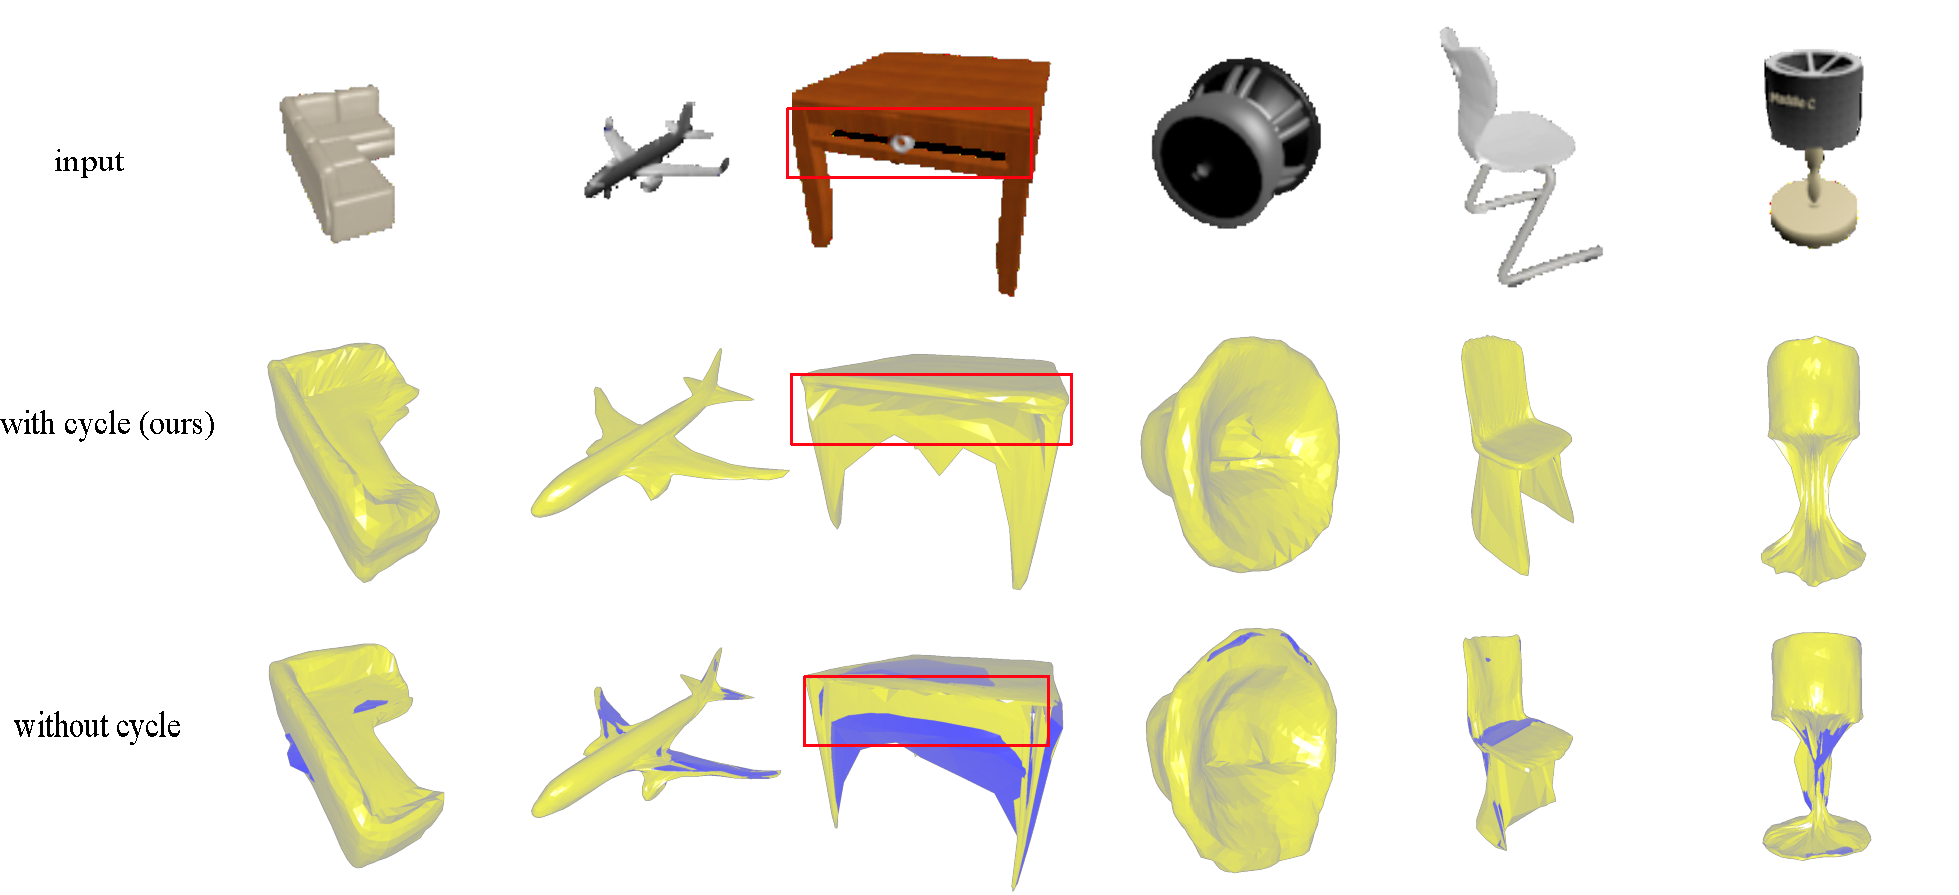
\includegraphics[width=\linewidth]{img/atlas/svr}
	\caption{Cycle regularization on AtlasNet: All the visualized cases here are selected from the test set of AtlasNet. Some meshes' view direction are manually adjusted to better expose the differences. The red rectangles are highlighting a case (the table) in which more details are preserved than the original network because we are enforcing the surface to be free of self-intersection with our cycle regularization term}
	\label{fig:svr}
\end{figure*}

\noindent{\textbf{Data}} To fairly evaluate the effect of cycle regularization, we use the datasets released by AtlasNet and Pixel2Mesh respectively. Their model sets are both subsets of ShapeNet\cite{shapenetdata} and they both used the rendered image from \cite{3DR2N2}. The absolute size and position of the models and the sampled points as ground truth are not processed in the same way in these two datasets, which makes it unreasonable to compare them all together. However, this doesn't prevent us to show the effect of our regularization technique separately.

\noindent{\textbf{Mesh generation and visualization}} Since we are addressing a issue regarding the quality of generated mesh, any post-processing used in AtlasNet\cite{atlasnet} are not used in our experiment. All the triangulations are directly transfered from the predefined surface. We do not divide the triangles to get denser vertex either. The meshes from AtlasNet all have 2500 vertices and about 4k faces. The meshes from Pixel2Mesh all have 2466 vertices and 4928 faces.

To better expose the issue we are addressing in this paper, we render the generated mesh in the software MeshLab and use the ``gooch.gdp" in the software as our shader. In such mode the triangles are rendered golden at front and bluish at back. The golden region and bluish region interlacing at surface evidently indicates the self-intersected triangles.

\noindent{\textbf{Evaluation criteria}}
In order to quantitatively evaluate the issue of self-intersection and self-overlap, we count the percentage of self-intersected triangles (``SI") over the total number of triangles. For this evaluation, we provide our code in the supplemental material which can calculate the ``SI" for a input mesh.  
We also use the value of Chamfer distance (``CD") as the original AtlasNet and Pixel2Mesh to evaluate how well the generated mesh approximate the target shape. For the evaluation of Chamfer distance we used the codes that are already implemented by AtlasNet\cite{atlasnet} and Pixel2Mesh\cite{pixel2mesh}.

\begin{table*}
	\caption{Test error on AtlasNet trained with(\textbf{ours}) and without cycle regularization. Chamfer distance(CD) and percentage of self-intersected(SI) faces are reported. ``AE" stands for the shape auto-encoding task, and ``SVR" stands for single view reconstruction task. Sphere means that the models are using sphere as predefined surface to sample points from. The mean is data-wise as it is implemented in the evaluation code of AtlasNet}
	\label{tab:atlas}
	\centering
	\begin{tabular}{c|rc|rc|rc|rc|}
		\multirow{2}{*}{CD,SI} &\multicolumn{4}{c|}{AE-sphere}&\multicolumn{4}{c|}{SVR-sphere}\\
		\cline{2-9}
		~& \multicolumn{2}{c|}{without-cycle} & \multicolumn{2}{c|}{ours} & \multicolumn{2}{c|}{without-cycle} & \multicolumn{2}{c|}{ours} \\
		\hline
		cellphone&1.3,&0.53\%&1.4,&3.4e-3\%&3.8,&1.4\%&3.7,&2.7e-4\%\\
		watercraft&1.5,&2.3\%&1.8,&6.8e-4\%&4.3,&7.4\%&4.3,&2.6e-4\%\\
		monitor&1.8,&1.8\%&2.0,&9.8e-4\%&6.9,&3.4\%&6.5,&9.8e-4\%\\
		car&1.8,&0.52\%&1.8,&8.0e-4\%&3.9,&0.47\%&3.8,&1.8e-3\%\\
		couch&1.9,&2.5\%&1.9,&8.8e-4\%&5.1,&2.0\%&4.9,&1.7e-3\%\\
		cabinet&2.0&2.3\%&2.2,&1.2e-2\%&5.3,&3.6\%&5.2,&4.3e-3\%\\
		lamp&2.7,&14\%&3.4,&5.5e-2\%&13.2,&19\%&13.1,&2.0e-2\%\\
		plane&1.0,&18\%&1.2,&1.9e-3\%&2.6,&18\%&2.6,&2.9e-3\%\\
		speaker&2.9,&0.77\%&2.9,&1.1e-3\%&10.2,&1.7\%&9.6,&3.1e-4\%\\
		bench&1.3,&11\%&1.6,&7.4e-3\%&4.0,&12.3\%&3.9,&1.6e-2\%\\
		table&1.7,&12\%&2.0,&2.1e-2\%&4.9,&10.7\%&4.8,&1.79e-5\%\\
		chair&1.9,&12\%&2.1,&2.7e-2\%&5.3,&10.9\%&5.3,&2.3e-2\%\\
		firearm&0.7,&4.9\%&0.9,&2.1e-3\%&2.2,&18.2\%&2.2,&1.2e-3\%\\
		\hline
		mean &1.7,&8.5\%&1.9,& 1.3e-2\% &5.2,&9.6\%&5.0,&1.2e-2\%\\
		
	\end{tabular}
\end{table*}

\subsection{Visualize deformation process}
\label{subsec:deform}
In this subsection, we visualize the deformation process, providing a more intuitive view into the effect of our cycle regularization term. Being free of self-intersection is a rather geometric prior for surface mesh than a semantic one, therefore for the visualization in this section we do not involve any semantic networks and show the effect of our proposed technique in a pure shape deforming manner. In other words, we optimize the same loss function as in Equ.~(\ref{equ:atlascycle}), but do not use semantic networks (neither ResNet-18\cite{resnet} nor PointNet\cite{pointnet}) to generate the latent shape representation $\mathbf{s}$. We treat $\mathbf{s}$ as 1024 free variables. We initialize the parameters $\theta_f,\theta_g,\mathbf{s}$ randomly and sample $X$ from sphere surface in this experiment. For optimizer, we use gradient descent. Under such setting, we are deforming a randmly initialized shape (probably start with self-intersection) to a target shape. As in Figure~\ref{fig:opt}, the case of two target shapes (downloaded from the Internet) are shown. In these two cases, after few iterations our cycle regularization term take effect. It not only keep the mapping injective in optimization but also correct the self-intersection from the initialization.

\begin{figure}[htbp]
	\centering
	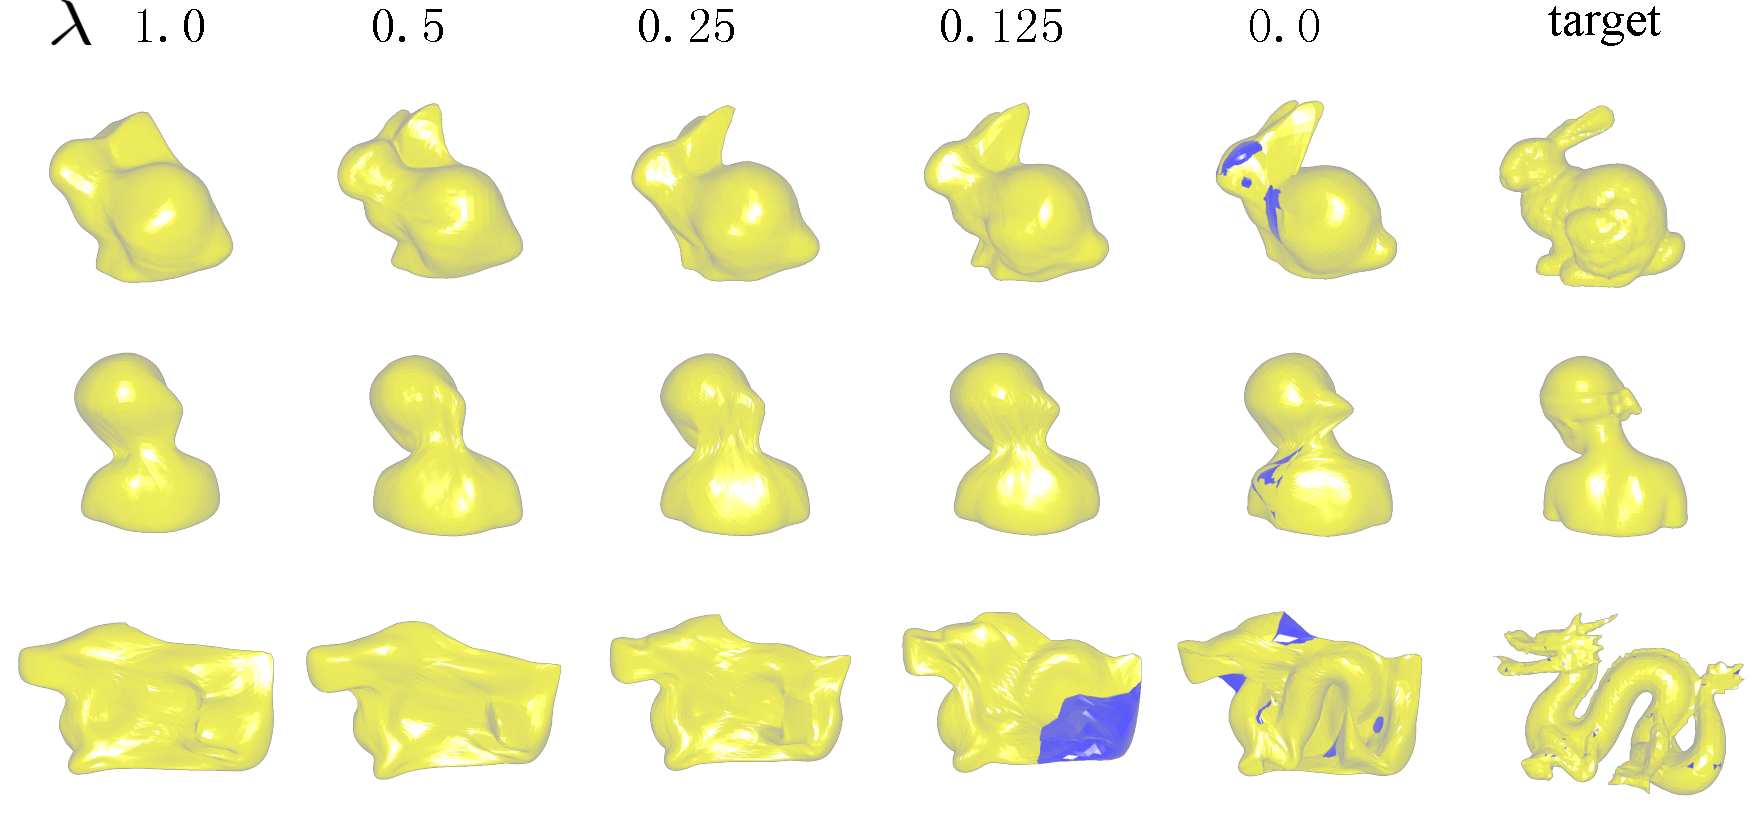
\includegraphics[width=\linewidth]{img/opt/lambda}
	\caption{The choice of $\lambda$: Under the setting in Sec~\ref{subsec:deform}, we show some results with different choice of $\lambda$}
	\label{fig:lambda}
\end{figure}

As shown in Figure~\ref{fig:lambda}, visually speaking, when set the weight $\lambda=0.25$, the deformed shape is able to approximate more details than the larger choices (i.e. $\lambda=0.5,1.0$), and it is also sufficient to enforce the injective mapping.  Therefore we use $\lambda=0.25$ as an emperical choice in following experiments, however finer tuning is possible depending on specific networks. 
\subsection{Cycle regularization with AtlasNet}
In this subsection, we show and discuss the effect of our cycle regularization term on  AtlasNet\cite{atlasnet}. As shown in Table~\ref{tab:atlas}, after applying our cycle regularization on the AtlasNet(sphere), the percentage of self-intersected triangles (``SI") are significantly reduced, while the Chamfer distance (``CD") remains close to original networks (somehow slightly worse in auto-encoding and better in single view reconstruction task). As visualized in Figure~\ref{fig:svr} for single view reconstruction task, the reduction of self-intersection is also visually evident. In some case, as highlighted by red rectangles in Figure~\ref{fig:svr}, our cycle regularization term even helps to improve the reconstructed details.
\subsection{Cycle regularization with Pixel2Mesh}

\todo{train and test Pixel2Mesh with and without cycle regularization}

\subsection{Limitations and future work}
When we apply our cycle regularization term to the model based on 25-patches, which is also released by AtlasNet\cite{atlasnet}, we encountered failure. We believe this is due to the reason we stated under \emph{Remaining gap} in Sec~\ref{subsec:cyclereg}. The AtlasNet based on 25-patches use 25 independent point-wise MLP to map the domain $[0,1]^2$ to different part of the target surface. This makes the overall mapping neither a canonical function (map one point from the patch to multiple points on surface) nor continue. In future, we want to try to use masks on continue domain instead of multiple patches to handle the case that the target surface is not homeomorphic to continue surface. This seems to be how the researchers usually handle it for human mouth on the face surface in parameterization. 
\section{Conclusions}
We propose the cycle regularization technique to .
%%\section*{References}
\bibliographystyle{named}
\bibliography{ParamNet}



\end{document}